\chapter{Combinatorial Game Theory}


\section{Basic Terminologies}

\begin{definition}
    \textbf{Games of chance} are games with a randomness component. i.e. a people's decisions do not entirely dictate their outcomes.
\end{definition}
\textbf{Example}:Roulette in the casino.


\begin{definition}
    \textbf{Games of partial information} are games where a player is not privy to all available information when making a turn.(no simultaneous movement)
\end{definition}
\textbf{Example}:Poker: a player does not know the cards of other opponent.


\begin{definition}
    \textbf{Sequential games} are games where players alternate turns one after the other.
\end{definition}
\textbf{Example}:A mordern video game, say GTA5 online, is a non-sequential game that everyone can move simultaneously.


\begin{definition}
    \textbf{Games of perfect information} are games where both players have access to all available information.
\end{definition}


\begin{definition}
    \textbf{Well-founded games} are games where after a finite number of turns, the game ends.
\end{definition}
\textbf{Remark}:
\begin{itemize}
    \item Chess is not well-founded since players can moving pieces back and forth.
    \item Fun fact: Mathematically speaking, no well-founded game is fair.
\end{itemize}

\noindent \textbf{Note}:
\begin{itemize}
    \item Games of chance and games of partial information lie mostly in the realm of probability theory and economics.(research initialed by J.Von Neumman and J.Nash) 
    We will mostly be interested in games where both players have perfect information, and the game inevitably must end.(Sadly, this leaves chess out, though there is some research in this regard.)
    \item We also stick with two player games, though the theory of n-player games can be reduced to two players (Assuming all $n-1$ other players are colluding and form a second player)
\end{itemize}


\section{Three Simple Games}

\noindent \textbf{Tic-Tac-Toe}\\

\textbf{Introduction}:
\begin{itemize}
    \item Tic-Tac-Toe is a game between two players that takes place on a three by three grid.
    \item Players take turns filling in the grid one square at a time.
    \item The first player only fills the grid with X's.
    \item The second player only fills with O's.
    \item The game ends when a player has taken three positions that form a line in the grid.
\end{itemize}
\begin{figure}[ht]
    \centering
    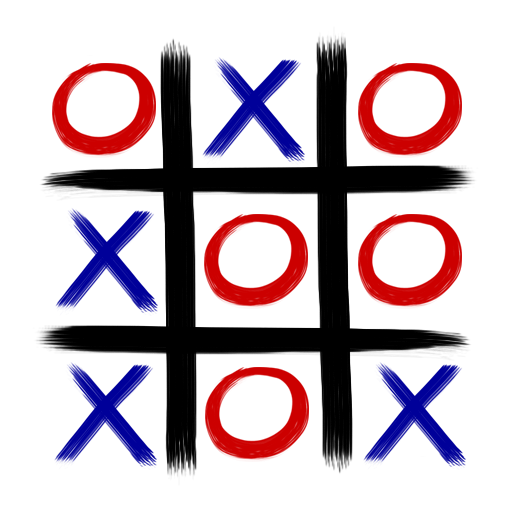
\includegraphics[scale=0.4]{Images/TicTacToe_HD_iTunesArtwork.png}
    \caption{A picture of tic-tac-toe}
\end{figure}

\textbf{Observation}:
\begin{itemize}
    \item It is a sequential game.
    \item The game is of perfect information.
    \item The game was played fast and well-founded.
    \item The first player was favoured.
    \item The game ties early.
    \item The only way that a player losses is if they make a mistake.
\end{itemize}


\noindent \textbf{Nim}\\

\textbf{Introduction}:
\begin{itemize}
    \item The set up is just three piles of stones. $(a,b,c)$ where each entry is apositive integer number of stones. $a,b,c \in \Z^+$
    \item Each turn, a player will pick a pile and remove any number of stones from that pile. For example, if it is player1's turn and the board state is $(5,2,0)$, then 
    $$(5,2,0) \longrightarrow (4,2,0)$$ $$(5,2,0) \longrightarrow (0,2,0)$$ $$(5,2,0) \longrightarrow (5,1,0)$$
    are all valid responses, but $(4,1,0)$ is not.
    \item The winning player is the one who drew the last stone.(Alternatively, the loser is the one with no stones to grab)
\end{itemize}
\begin{figure}[ht]
    \centering
    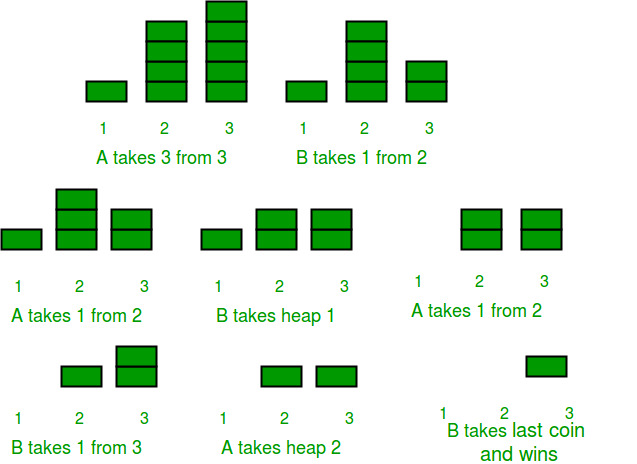
\includegraphics[scale=0.4]{Images/game3-2.jpeg}
    \caption{An example of Nim}
\end{figure}

\textbf{Observation}:
\begin{itemize}
    \item It is asequential game.
    \item The game is of perfect information.
    \item The game is well-founded and appears to be decided early.
    \item The nim depends on the initial pile.
    \item The first player seems to have advantage.
    \item The game is symmetric.
    \item The moment when we force two equal piles, the game is over.
    \item Nim always has a winner.
\end{itemize}


\noindent \textbf{The N-Gale-Stewart Game}\\

\textbf{Introduction}:
\begin{itemize}
    \item Let $A$ be a subset of length $N$ binary strings.
    \item Two players take turns picking either 0 or 1.
    \item The game terminates when the string hits length $N$.
    \item Player1(Alice) wins if the created string $s \in A$. Else, player2(Bob) wins.
\end{itemize}


\section{Formalizing Game}

\begin{definition}
    A \textbf{game} $\mathcal{G}$ between two players 1 and 2 is a collection of rules.
\end{definition}

\begin{definition}
    A \textbf{run/play} of the game is string of alternating moves $x_iy_i$ between player1 and player2.
\end{definition}

\begin{definition}
    Each player has a disjoint set $A_1$ and $A_2$ of terminal runs of the game called \textbf{payoff sets}.
\end{definition}

\begin{definition}
    We say player1 \textbf{wins a run} if and only if a run of the game $s \in A_1$ and similarly for player2.
\end{definition}
\textbf{Example}: For a Nim starts at the state $(3,4,4)$, for the game that we played in the class, we have a string 
$$(0,4,4) \cdot (0,2,4) \cdot (0,2,2) \cdot (0,0,2) \cdot (0,0,0)$$ This string would be inside player1's payoff set $A_1$.

\begin{definition}
    \textbf{Game states} are strings $s$ where $\forall i \in \N. s(2i-1)=x \text{ and } s(2i)=y_i$.
    We consider the empty string $\emptyset$ as the start of the game.
\end{definition}
\textbf{Remark}:
\begin{itemize}
    \item Sequence/string generally are interchangeable in mathematics, but we stick with the notion of string as they're finite most of the time and we don't want to mix-up/confuse you with sequences from analysis (which on the flipside are almost always presumed to be infinite).
    \item Game state refers to the strings s, places the game COULD go. Run usually is reserved for terminal game states i.e the strings t where the game has ended. 
\end{itemize}

\begin{definition}
    We call a game $\mathcal{G}$ \textbf{well-founded} if every possible run of the game ends after finitely many turns. We say it is \textbf{ill-founded} if it is not well-founded.
\end{definition}

\begin{definition}
    Given a game $\mathcal{G}$, \textbf{the game tree} $T_{\mathcal{G}}$ is the poset of all possible game states. We say $s \leq_{\mathcal{G}} t$ if for all $i$ in the domain of $s$, $s(i)=s(t)$. 
    When we dipict the game tree, we always mean the cover graph of $T_{\mathcal{G}}$ (Note, the cover graph will always be a tree, hence the name)
\end{definition}
\begin{figure}[ht]
    \centering
    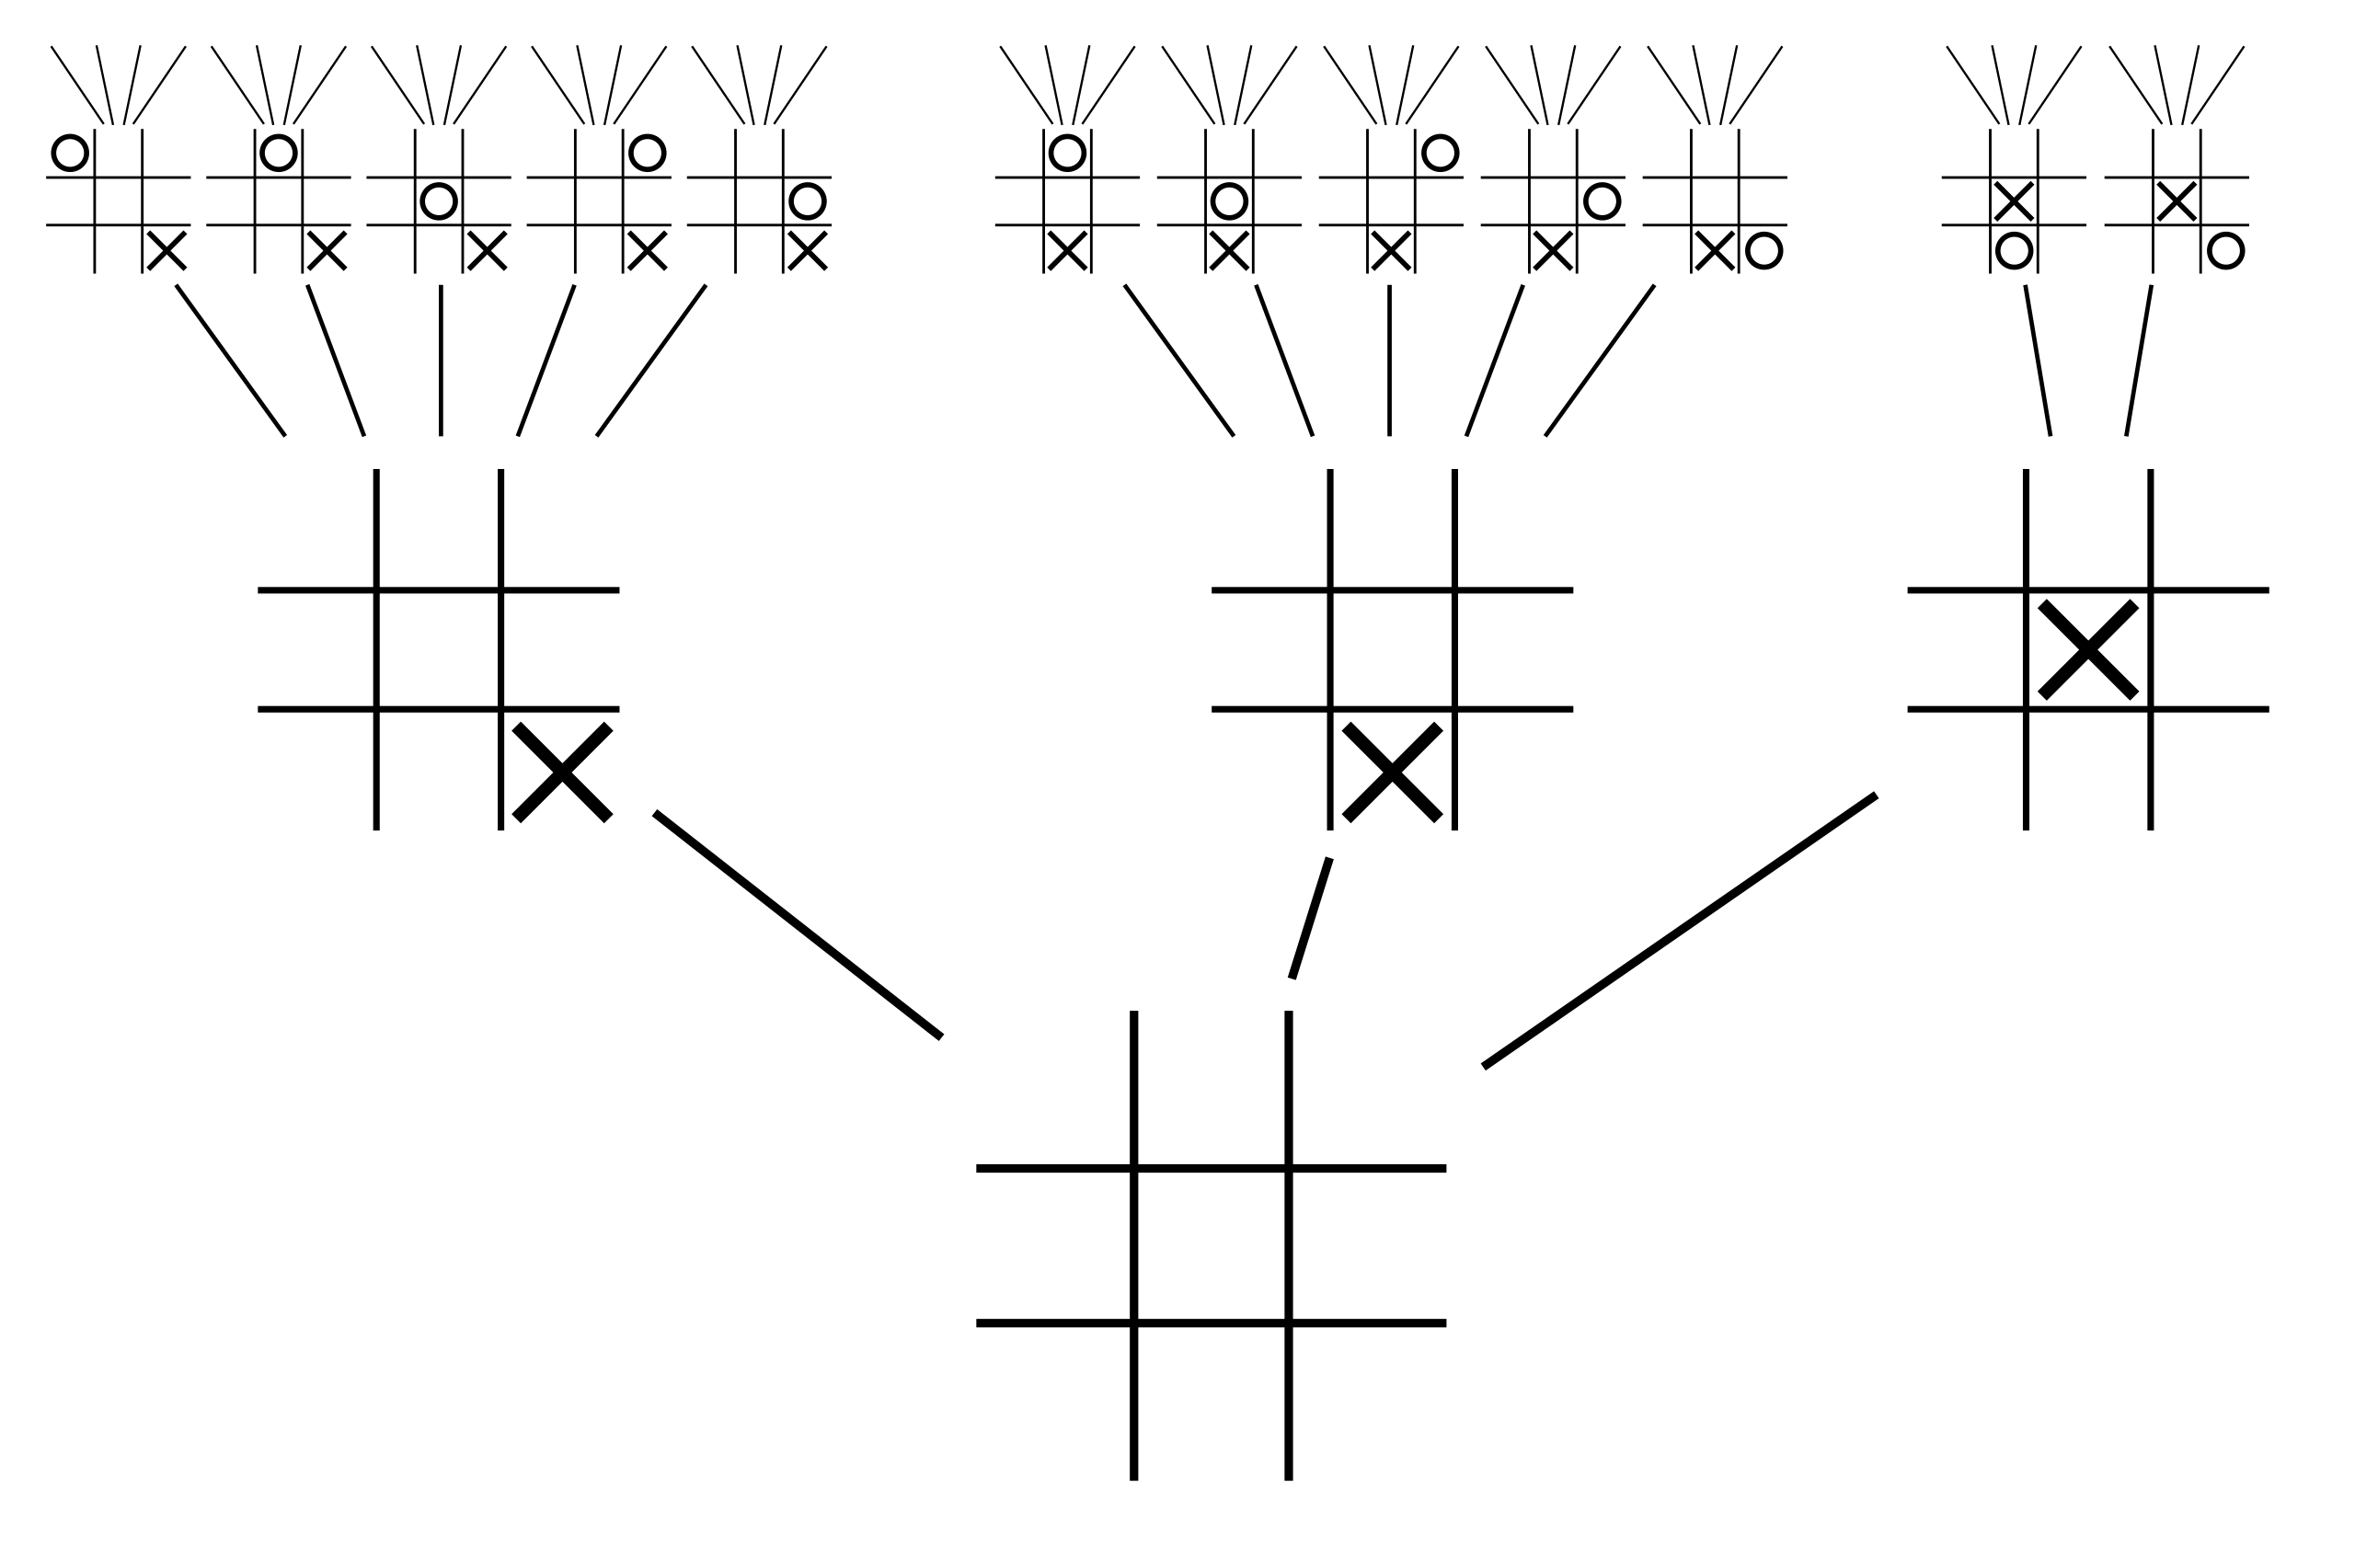
\includegraphics[scale=0.1]{Images/Tic-tac-toe-game-tree.svg.png}
    \caption{Incomplete game tree of tic-tac-toe}
\end{figure}





\section{Strateries for Games}

\noindent \textbf{What is strategy?}
\begin{itemize}
    \item A colletion of responses to a particular outcome.
    \item A response to acurrent game state that gets close to a payoff state.
\end{itemize}

\begin{definition}
    Let $\mathcal{G}$ be a game between Alice and Bob.(Alice goes first). 
    A \textbf{strategy} for Alice is a function $f$ that takes game state $s$ of length $2n$ and returns a game state $f(s)$.
    $$f:s \longrightarrow f(s)$$
    where $length(f(s))=2n+1$ and $s \leq_{\mathcal{G}} f(s)$.i.e. it provides a response to any move Bob can make in any situation.
\end{definition}
\textbf{Remark}:
\begin{itemize}
    \item A strategy for Bob is defined symmetrically.
\end{itemize}

\textbf{Example}:
\begin{itemize}
    \item \textbf{The mirroring strategy} for Bob is playing whatever Alice played.
    \item \textbf{The zero strategy} for Bob is always picking zero.
\end{itemize}

\begin{definition}
    Given a game $\mathcal{G}$, we call a strategy \textbf{winning} if whether the player uses it, he win.
\end{definition}
\textbf{Example}:
Consider the 4-Gale-Stewart game with payoff set $A=\{0101,0001,0100,0000\}$
\begin{itemize}
    \item The zero strategy for Alice is winning.
    \item The mirroring strategy for Bob is not winning.
\end{itemize}

\begin{theorem}[The first strategy theorem]
    Given a game $\mathcal{G}$, both Alice and Bob cannot have a winning strategy.
\end{theorem}
\begin{proof}
    Let $f$ be the winning strategy of Alice, and let $g$ be the winning strategy of Bob. 
    Play a run of the game where Alice plays according to $f$ and Boo plays according to $g$. 
    Since $f$ is winning, Alice wins. Since $g$ is winning, Bob wins. 
    This is a contradiction, games can only hane one winner.
\end{proof}

\begin{definition}
    Given an integer $n$, it's associated \textbf{binary representation} is the unique sequence $a_k \in \{0,1\}$ (from right to left) with the property that $$n=\sum_{k=0}^na_k\cdot 2^k$$
\end{definition}

\begin{definition}
    Given two binary strings $s$ and $t$, the \textbf{nim-sum} $$s \oplus t$$ 
    is the binary string $r$ where $$r(i)=0 \text{ iff } s(i)=t(i)$$
\end{definition}
\textbf{Example}:
\begin{itemize}
    \item $111 \oplus 101=010=10$
    \item $1110000 \oplus 1111 = 1110000 \oplus 0001111=1111111$
    \item $10101 \oplus 10101=000000=0$
\end{itemize}

\begin{theorem}[Properties of nim-sum]\
    \begin{itemize}
        \item $s \oplus t = t \oplus s$
        \item $(s \oplus t) \oplus r = s \oplus (r \oplus t)$
        \item $s \oplus 0=s$
        \item $s \oplus t =0 \text{ iff } s=t$
    \end{itemize}
\end{theorem}
\textbf{Remark}:
\begin{itemize}
    \item Let $\{0,1\}^+$ denotes $\{0,1\}^*-\{\lambda\}$. 
    Let $\forall x \in \{0,1\}^+.i(x)=x$\\
    Then $(\{0,1\}^+, \oplus, 0, i)$ is a group, futher, am abelian group.
    \item From the algebraic perspective, the last property means that in this abelian group, the inverse of x is x itself.
    \item The essense of nim-sum:
    \item \begin{itemize}
        \item if the nim-sum of two piles equals zero, then the two piles have the same amount of stones.
        \item if the nim-sum of three piles equals zero, then the amount of stones in the largest pile equals to the sum of stones in the other two smaller piles.
    \end{itemize}
\end{itemize}

Informally, we can define an \textbf{equilibrium state} when the amount of stones in the largest pile equals the amount of stones in the other two piles.\\

If we played the game some times, we will notice:
\begin{itemize}
    \item if we are at an equilibrium state, then whatever we do, the next state is not equilibrium.
    \item if we are at a non-equilibrium state, then we can do something to make the next state equilibrium.
\end{itemize}
We can formalize our observation to make the following lemmas.

\begin{lemma}
    Suppose in a game of Nim, the piles have $s_1,s_2,s_3$ many stones where the number is written in binary. 
    If $s_1 \oplus s_2 \oplus s_3=0$, then after any move to the board state $t_1,t_2,t_3$, we have $t_1 \oplus t_2 \oplus t_3 \neq 0$
\end{lemma}
\begin{proof}
    Suppose $s_1 \oplus s_2 \oplus s_3=0$. 
    Suppose without loss of generality, we remove some number from the first pile $s_1$. 
    So the board state is now $t_1,s_2,s_3$. 
    We claim that there is a non-zero $r$ such that $s_1=t_1 \oplus r$. 
    (if $r=0$, then $t_1=s_1$ and we removed nothing) 
    By way of contradiction, suppose $t_1 \oplus s_2 \oplus s_3=0$.
    It follows that 
    \begin{equation}
        \begin{split}
            s_1 \oplus s_2 \oplus s_3 &= (r \oplus t_1) \oplus s_2 \oplus s_3\\
            &= r \oplus (t_1 \oplus s_2 \oplus s_3)\\
            &= r \oplus 0\\
            &= 0
        \end{split}
    \end{equation}
    Hence $r=0$, this is a contradiction.
\end{proof}



\begin{lemma}
    Suppose $s_1,s_2$ and $s_3$ is the current board state in a game of Nim, and $$s_1 \oplus s_2 \oplus s_3 \neq 0$$
    Then there is a move that can be made to the board state $t_1,t_2,t_3$ such that $$t_1 \oplus t_2 \oplus t_3=0$$
\end{lemma}
\begin{proof}
    Since $s_1 \oplus s_2 \oplus s_3$ is non-zero binary string. 
    Then the string $s_1 \oplus s_2 \oplus s_3$ has a leading 1. 
    Assume the leading 1 is at the i-th spot from right to left. 
    It follows that one of one of $s_1,s_2,s_3$ has a 1 in the i-th spot. 
    (either 3 of them have ones or just one of them has a one in the i-th spot)
    Without loss of generality, suppose it is $s_1$. We claim that $s_1 \oplus (s_1 \oplus s_2 \oplus s_3)$ is less than $s_1$.
    \begin{equation}
        \begin{split}
            s_1 \oplus (s_1 \oplus s_2 \oplus s_3) &= (s_1 \oplus s_1) \oplus s_2 \oplus s_3\\
            &= 0 \oplus s_2 \oplus s_3\\
            &= s_2 \oplus s_3
        \end{split}
    \end{equation}
    By assumption, all spots on the left side of the i-th spot of $s_2 \oplus s_3$ must be the same as the corresponding spots of $s_1$. 
    For the i-th spot, $s(i)=1$ and $s_2 \oplus s_3(i)=0$. It suffices to conclude that $s_2 \oplus s_3 <s_1$.
    Remove blocks from $s_1$, make $t_1=s_1 \oplus (s_1 \oplus s_2 \oplus s_3)=s_2 \oplus s_3$. 
    It follows that the nim-sum of the three piles is now 
    \begin{equation}
        \begin{split}
            t_1 \oplus s_s \oplus s_3 &= (s_2 \oplus s_3) \oplus s_2 \oplus s_3\\
            &= (s_2 \oplus s_3) \oplus (s_2 \oplus s_3)\\
            &= 0
        \end{split}
    \end{equation}
\end{proof}


\begin{theorem}[Winning strategy for Nim]
    Let $s_1,s_2$ and $s_3$ be the starting board state of a game of Nim. 
    If $s_1 \oplus s_2 \oplus s_3 \neq 0$, then the player1(Alice) has a winning strategy. Else, player2(Bob) has a winning strategy.
\end{theorem}
\begin{proof}
    Suppose $s_1 \oplus s_2 \oplus s_3 \neq 0$. 
    Let Alice play with the strategy that she always moves so that the following board state satisfies $t_1 \oplus t_2 \oplus t_3 =0$. 
    By the second lemma, such a move is always possible. By the first lemma, no matter what move Bob makes, the nim-sum will be non-zero(hence we can make the nim-sum zero) 
    Since the total number of stones is finite and it decreases each turn. Hence the game must terminate. 
    Note, when it ends, the nim-sum of the piles must be zero. 
    Hence it was Alice that made the last move and she wins. 
    If $s_1 \oplus s_2 \oplus s_3=0$, any move Alice makes will make the nim-sum of thr pile non-zero. 
    Bob then canplay with Alice's strategy which symmetically is winning.
\end{proof}


\section{Determinism}


\begin{definition}
    we say a game $\mathcal{G}$ is \textbf{determined} if one of the players has a winning strategy.
\end{definition}
\textbf{Remark}:
\begin{itemize}
    \item We now know Nim is determined.
\end{itemize}

\begin{theorem}[N-Gale-Stewart is determined]
    For every subset of length $N$ binary strings $A$, the N-Gale-Stewart game where Alice has payoff set $A$ is determined.
\end{theorem}
\begin{proof}
    By induction on $N \in\N$\\
    Base case: The only strings of length 1 are 0 and 1.
    \begin{itemize}
        \item If $A \neq \emptyset$, then Alice has a winning strategy since she can simply choose 1 or 0 depending on which is in $A$.
        \item If $A = \emptyset$, then Bob has a winning strategy since no matter what move Alice makes, doing nothing can win.
    \end{itemize}
    Inductive step: Suppose the N-Gale-Stewart game is determined for any payoff set. 
    Consider an (N+1)-Gale-Stewart game. Let $A$ be the payoff set for Alice. Let $A'$ be the set of $N$ length binary strings defined by:
    \begin{itemize}
        \item For all $x \in A$, we have a prefix of $X$ with lengh $N$.
        \item We call this prefix $p$ and we put $p$ in the set $A'$.
    \end{itemize}
    \begin{figure}[ht]
        \centering
        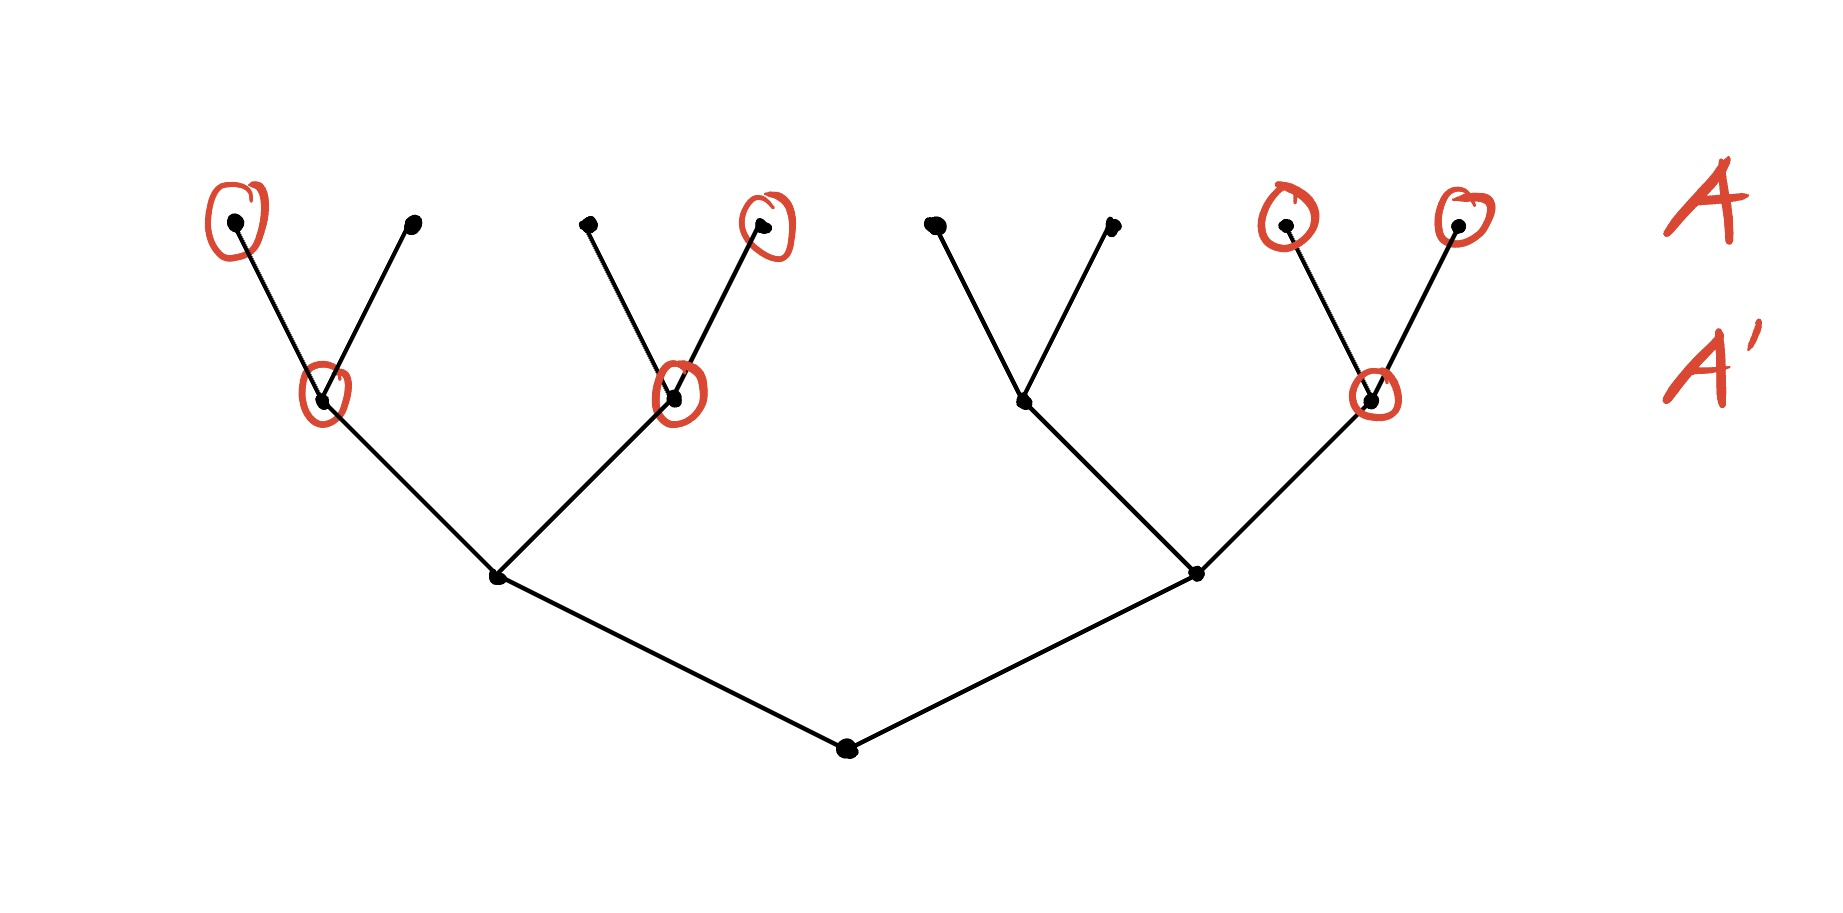
\includegraphics[scale=0.15]{Images/IMG_0295.jpg}
        \caption{An example of definining $A'$}
    \end{figure}
    So by our definition, any $p \in A'$ is $\leq_{\mathcal{G}}$-below some string in $A$.
    Now we can define a subgame: A N-Gale-Stewart game with payoff set for Alice $A'$. 
    By the induction hypothesis. This subgame is determined. 
    Hence one of Alice and Bob has the winning strategy. Without loss of generality, assume Alice makes the last move for the (N+1)-Gale-Stewart game. 
    Hence Bob makes the last move for the subgame. 
    \begin{itemize}
        \item If the winning strategy for the N-Gale-Stewart subgame is for Alice and she using that strategy during the game. Hence whatever the letter Bob choose, the string $p$ the make, is in $A'$. Then Alice can choose the last digit of the corresponding $X$ in $A$. 
        Therefore, Alice has a winning strategy a winning strategy for the (N+1)-Gale-Stewart game.
        \item If the winning strategy for the N-Gale-Stewart subgame is for Bob and he using that strategy during the game. Hence the string $p$ they make, is in $\{0,1\}^N-A'$. So whatever letter that Alice choose, the string $x$ they make is in $\{0,1\}^{N+1}-A$. Hence Bob wins. 
        Therefore, Bob has a winning strategy for the (N+1)-Gale-Stewart game.
    \end{itemize}
\end{proof}
\textbf{Remark}:
\begin{itemize}
    \item The strategy is sometimes called \underline{backtracking}, as we've trying to reverse a win from terminal game states.
\end{itemize}

\begin{theorem}[Zermelo's Theorem]
    Let $\mathcal{G}$ be a game with a well-founded game tree. Suppose every run of the game ends in a winner.(i.e. ties are not possible) Then a player has a winning strategy.
\end{theorem}
\begin{proof}
    Assume the game is finite. 
    We are going to apply the backtracking algorithm recursively.
    \begin{itemize}
        \item Start with the strings with the largest length. Colour them blue if Alice wins and red if Bob wins.
        \item Move down to the previous length strings. Without loss of generality, suppose it is Alice's turn. Colour the string blue if Alice can move to a blue string and red if all moves are red. (This step is symmetric for Bob)
    \end{itemize}
    Eventually, the empty string $\emptyset$ will be coloured. We claim that:
    \begin{itemize}
        \item If the colour is blue, then Alice has a winning strategy.
        \item If the colour is red, then Bob has a winning strategy.
    \end{itemize}
    Without loss of generality, suppose $\emptyset$ is blue. Alice will apply the strategy cotinuously:
    \begin{itemize}
        \item Alice can then choose a move to a game state coloured blue. Alice will play with the strategy of pickinga blue game state.
        \item Given Alice has chosen a game state that is coloured blue. On Bob's turn, it must be the case that all Bob's moves lead to game states that are coloured blue.
    \end{itemize}
    The game must terminate. When it does, Alice's strategy garantees the terminal state is blue. 
    By way we coloured the tree, a blue terminal game state means Alice wins.
\end{proof}

\begin{theorem}[Zermelo's Full Theorem]
    Let $\mathcal{G}$ be a game with a well-founded game tree, Then either the game is determined, or both players have strategies that either sin or force a tie.
\end{theorem}
\begin{proof}
    Consider the new games $\mathcal{G}_A$ and $\mathcal{G}_B$.
    \begin{itemize}
        \item $\mathcal{G}_A$ is played the same way as $\mathcal{G}$, but Alice wins as long as we do not reach Bob's payoff set.(i.e. if tiedin $\mathcal{G}$, then Alice wins)
        \item $\mathcal{G}_B$ is defined symmetrically.
    \end{itemize}
    Neither $\mathcal{G}_A$ nor $\mathcal{G}_B$ have ties, by the last theorem, they are determined.
    \begin{itemize}
        \item If $\mathcal{G}_A$ is determined in favour of Bob, then the strategy for Bob in this game is winning in $\mathcal{G}$.
        \item If $\mathcal{G}_B$ is determined in favour of Alice, then the strategy for Alice is winning in $\mathcal{G}$.
        \item Suppose Alice has a winning strategy in $\mathcal{G}_A$ and Bob has a winning strategy in $\mathcal{G}_B$. Then playing with Alice's strategy in $\mathcal{G}_A$ means BOb cannot win. similarly for Bob's. Hence, playing the strategies against one another in $\mathcal{G}$ forces a tie.
    \end{itemize}
\end{proof}
\textbf{Remark}:
\begin{itemize}
    \item Very naively, this suggests every well-founded game is in one of two forms. 
    A game like Nim which is favoured for somebody, or a game like tic-tac-toe where two perfect players always force a tie.
\end{itemize}

\noindent \textbf{Some words beyond}:\\
Consider the game Go:
\begin{itemize}
    \item The usual board is a 19 by 19 square with players either placing black or white pieces on the board.
    \item By our definition, the game Go is of perfect information and well-founded.
    \item By the Zermelo's full theorem: either Alice or Bob has a winning strategy, or two perfect player will end in a draw.
    \item Therefore, for any player that goes first in Go, he has a strategy that never lose theoretically.
\end{itemize}
Unfortunately, although the prof of Zermelo's theorem is constructive, the construction process requires us to get the whole game tree first. 
But in a game like Go, the number of terminal states is more than the number of atoms in the universe. It is impossible for now to get such strategy using this theorem.



\section{Infinite Games}

\begin{definition}
    A game is \textbf{ill-founded} if there are infinite runs.
\end{definition}
\textbf{Remark}:
\begin{itemize}
    \item Infinite runs tend to be the feature of infinite games, making our tools like Zermelo's theorem and methods like backtracking futile.
\end{itemize}


\begin{definition}
    The \textbf{Gale-Stewart game} is played as follows:
    \begin{itemize}
        \item Alice has some payoff set $A$ of infinite binary strings $s:\N \longrightarrow \{0,1\}$.
        \item Alice and Bob take turns choosing either 0 or 1.
        \item Alice wins if the created string is in $A$ and Bob wins otherwise.
    \end{itemize}
\end{definition}

\begin{lemma}
    If the payoff set $A$ for Alice is finite in the Gale-Stewart game, then Bob has a winning strategy.
\end{lemma}
\begin{proof}
    Suppose $A=\{s_1,s_2.\cdots,s_k\}$. Bob will play with the strategy that on his i-th turn, he will pick 0 if $s_i(2i)=1$ and pick 1 otherwise. 
    On the rest of Bob's turn after his k-th turn, he will only pick 0. 
    Bob's strategy ensures that the terminal sequence $s$ satisfies the condition $s(2i) \neq s_i(2i)$ and hence $s \notin A$.
\end{proof}
\textbf{Remark}:
\begin{itemize}
    \item This is like the diagonalization proof.
    \item We can generalize the lemma to the situation that $A$ is countable.
\end{itemize}


\begin{theorem}[*]
    There is a set of binary string $A$ such that neither Alice nor Bob has a winning strategy in the Gale-Stewart game with payoff set $A$ for Alice.
\end{theorem}


\begin{definition}
    The \textbf{Kubis' Game(for Graphs)} is defined as follows:
    \begin{itemize}
        \item The game is between Alice and Bob.
        \item The game starts with the emptygraph $(\emptyset, \emptyset)$.
        \item On each player's turn, if the current graph is $(V,E)$, the player responds by adding new vertices $X$ and edges strictly between vertices in $X$ and $X \cup V$.(i.e. a player cannot add edges where there weren't any previously)
        \item Say Alice wins for a graph $K$ if in a run she can create a graph isomorphic to $K$.
    \end{itemize}
\end{definition}


\begin{lemma}
    If there us a graph $K$ for which Alice has a winning strategy, it must contain every finite graph as a subgraph.
\end{lemma}
\begin{proof}
    Fix a graph $G$. Let Alice play with her strategy. 
    Let Bob play with the strategy that on his turn, he always adds a disjoint copy of G. 
    Since Alice's strategy is winning, the final graph will be isomorphic to $K$. 
    By Bob's strategy, the graph will have infinitely many disjoint copies pf $G$ as a subgraph. 
    Since $G$ was arbitrary, this is true for any finite graph $G$.
\end{proof}

\begin{theorem}[*Erdos-Rado]
    There is an infinite graph $R=(V,E)$ which can be expressed as an $\N$ indexed union of finite graphs with the property that for every pair of finite disjoint vertex set $V_1$ and $V_2$, 
    there is a $v \in V$ which is adjacent to everything in $V_1$ and nothing in $V_2$. 
    Moreover, any infinite graph with this property is unique up to isomorphism.
\end{theorem}


\begin{theorem}
    There is a winning strategy for Alice for $R$ in the Kubis' game.
\end{theorem}
\begin{proof}
    Let Alice play with the strategy that on her turn, if the current graph is $(V,E)$, for any subset $A \subset V$, 
    she responds by adding vertex $v_A$ such that $v_A$ is connected to everything in $A$ and not connected to anything outside of $A$. 
    Suppose at the end of the game, we have an infinite graph $R$. 
    Take arbitrary subsets of vertices $V_1$ and $V_2$ such that $V_1.V_2$ disjoint. 
    At some stage of the game, all the vertices of $V_1$ and $V_2$ just appeared. 
    Shortly after, on Alice's turn, she added a vertex who's neighbours were $V_1$ and shared no edges with $V_2$. 
    It follows that this graph is isomorphic to $R$>
\end{proof}